
\chapter{Optical-Based Shape Modeling}
\label{shape_modeling}
%\title{Shape from Silhouette Method for Approach Shape Modeling in Visual and Infrared}
\begin{document}
\section{Introduction}

In this work, the models presented are generated from both simulated and actual mission data sources and compared to the most resolute shape models available for the bodies in question. The method is tested on both a convex and irregular body in order to show how our overlaid silhouette trimming procedure responds to self-shadowing, the presence of concavity, as well as phase angles  projections introduced by the orientation of the sun and camera. This work will be developed as necessary to enable onboard shape model generation, but this paper serves to present and defend the method which uses a process of refinement based on extending the shape along the silhouette cutout in space, and narrowing down the three-dimensional hull through multiple view angles. As the small body community looks to grant more SIMPLEx level missions to asteroids, such as the Janus mission which will rendezvous with a binary system, it is necessary to develop the autonomous onboard navigation capabilities that make those missions possible. 

\section{Methods}
\subsection{Assumptions} 
In it's current formulation, this shape modeling method processes a batch of optical and infrared images taken at a reasonable distance away from a target body. The body does not need to be centered in the frame of the image, nor does it need to be fully lit. The assumptions made in the work to follow include full knowledge of the body frame, beginning with the orientation of the spin pole and further defined by convention. The orientation and location of the camera is known along with its frame, as well as the sun location in the body frame. In actual missions, there is a reasonable track of the spacecraft orientation and location in the inertial (sun-centered) frame, and a state estimate is formed for the body during approach and during ground-based observation campaigns. In this work, perfect certainty of the body location, spacecraft location, and the camera-pointing vector can be assumed.    

\subsection{Simulated Image Procedure}
Simulated images were necessary to test the robustness of our modeling method. The process of generating these images was performed via Blender software {blender} with the goal of recreating conditions of the OSIRIS-REx approach phase to the asteroid Bennu. The shape model was of 6m resolution, sourced from the approach data results given by the OSIRIS-REx mission{Lauretta2019}. Lighting conditions, such as the sun location, were manipulated to match the testing criteria but the inherent qualities were kept constant: a light strength of 5 MW, $0\%$ specularity, and a radius of 1m were suitable to illuminate the target for the purpose of recreating mission-similar conditions. Both a regular and irregular body were tested. The camera dimensions were kept in accordance with the PolyCam on the OSIRIS-REx mission{Rizk2017}.
%insert table outlining PolyCam camera parameters that you had to put into Blender (just fov? also image size/resolution?)



\subsection{Mission Data}
\begin{wrapfigure}[21]{R}{0.5\textwidth}
    \centering
    \captionsetup{justification=centering}
     \begin{subfigure}{0.23\textwidth}
         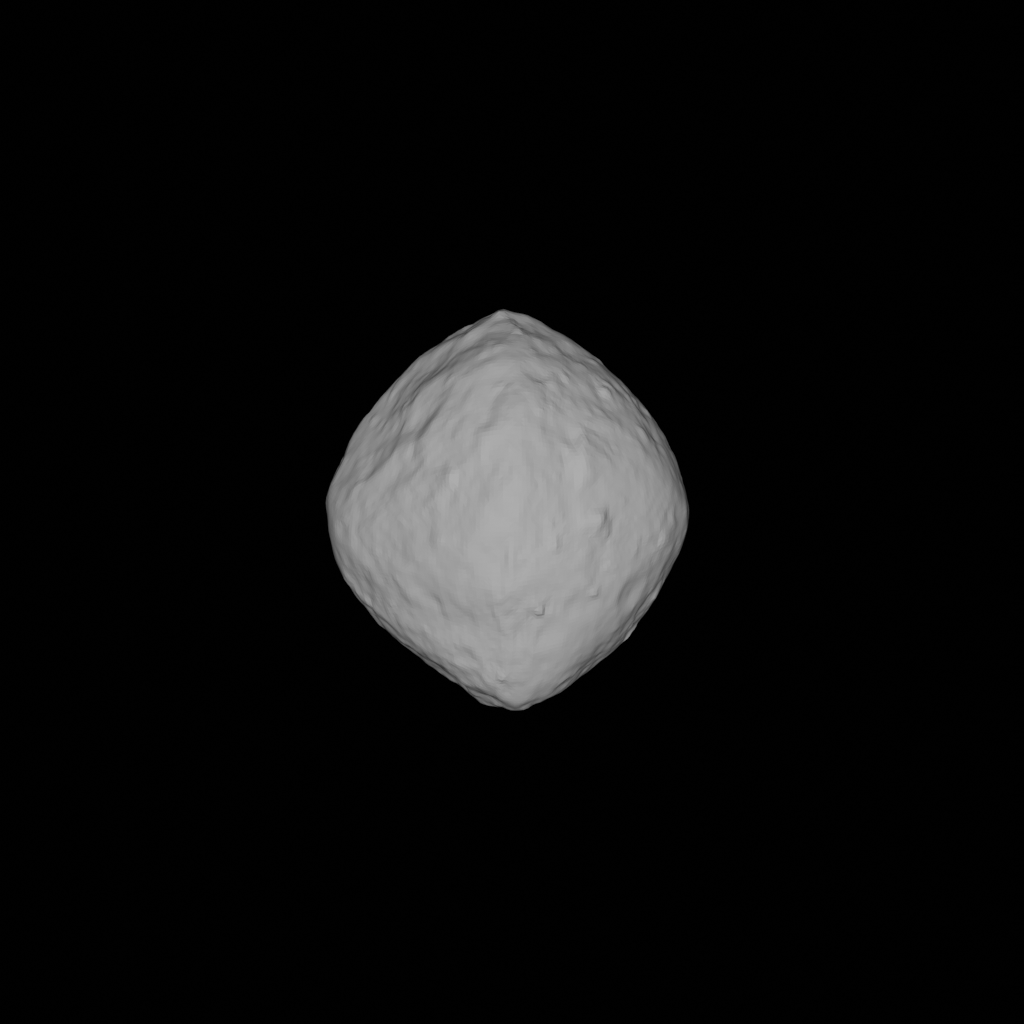
\includegraphics[width =\textwidth, height = \textwidth]{fig/render72.png}
         \caption{Simulated Bennu in Blender}
         \label{fig:y equals x}
     \end{subfigure}
    \hfill
     \begin{subfigure}{0.23\textwidth}
         \centering
         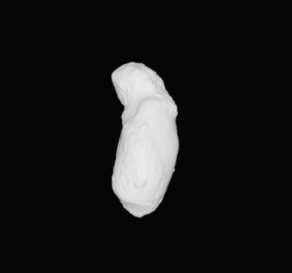
\includegraphics[width = \textwidth, height = \textwidth]{fig/Screen Shot 2021-02-18 at 11.43.43 AM.png}
         \caption{Simulated Itokawa in Blender}
         \label{fig:three sin x}
     \end{subfigure}
     
     \begin{subfigure}{0.23\textwidth}
         \centering
         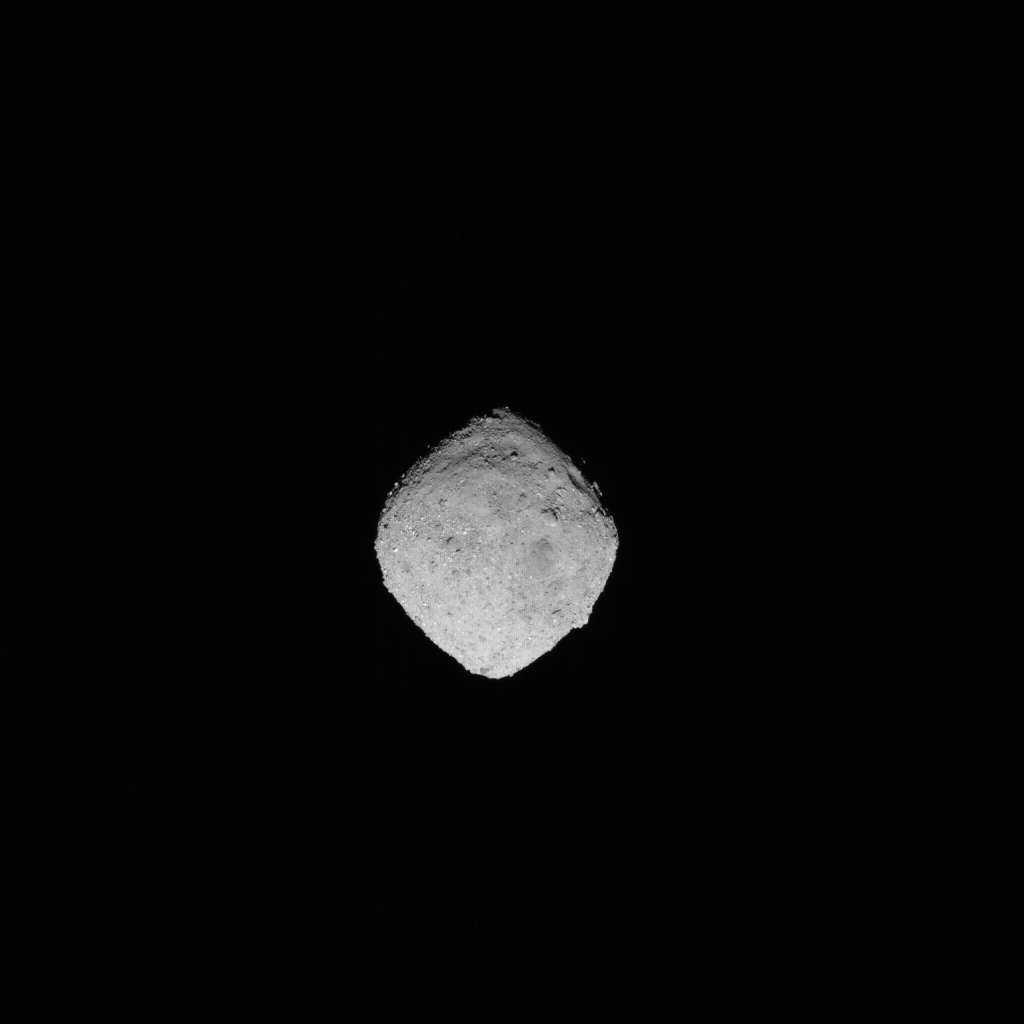
\includegraphics[width=\textwidth, height = \textwidth]{fig/image_69.png}
         \caption{OSIRIS-REx Mission Image}
         \label{fig:y equals x}
     \end{subfigure}
    \hfill
     \begin{subfigure}{0.23\textwidth}
         \centering
         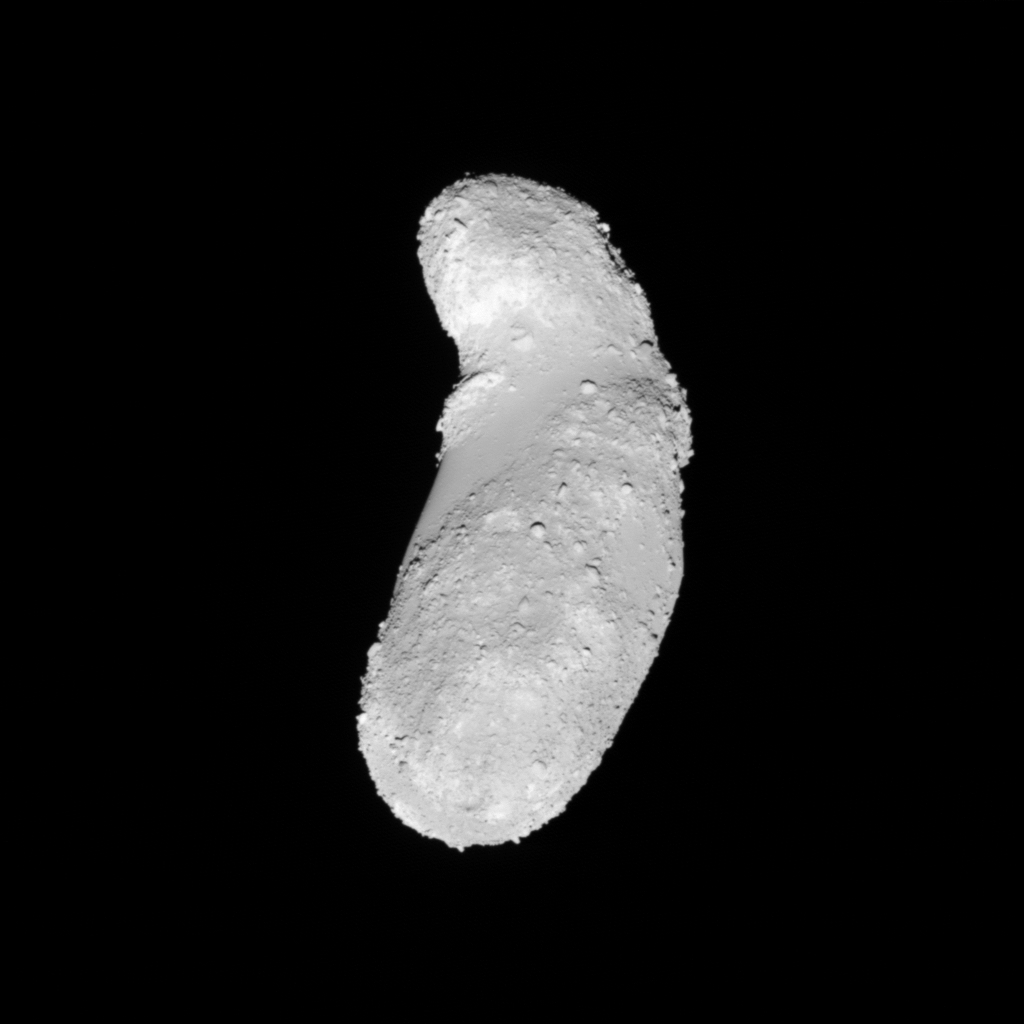
\includegraphics[width=\textwidth, height = \textwidth]{fig/st_2423026558_v.png}
         \caption{Hayabusa Mission Image}
         \label{fig:three sin x}
     \end{subfigure}
        \caption{Example Images}
        \label{fig:four_images}
\end{wrapfigure}
The data obtained to further test the modeling software was sourced from the OSIRIS-REx and Hayabusa mission SPICE archives. Necessary data regarding the camera dimensions, frame-to-frame transformations, the state of the camera, body, and sun were accessed as well as the images themselves which came from the PDS archives but their timestamps allowed for coordination of state and image. Shown below is an example of similarity between the simulated image sets and actual mission data, which proves that moving forward with both can provide comparable results when focusing on the silhouette information.



\subsection{Image Processing - Finding the Silhouette}

The procedure of shape generation using optical data begins with processing the images and finding the desired information - the silhouette of the body. The data shows results where the camera is within 100km, 151km, and 8km of the target body for the simulated test cases, the OSIRIS-REx data, and the Hayabusa images respectively. Examples of the input are shown in Fig. \ref{fig:four_images}. The simulated images and the mission data differ most in their surface detail, where rocks and boulders can be seen readily on mission images but are majorly missing from the surface representations of the shape models processed by Blender. For the purposes of silhouette-based shape modeling, this detail is acceptable and there are many steps implemented to ensure that all data sets are treated equally. This algorithm begins with a pre-processing thresholding procedure. An image is translated from RGB values into grayscale between [0,255] in intensity. These values are then flattened with the lowest intensity pixels ($< 2$) removed and all other intensities amplified by a factor of 1000. This produces a flat background of space with a bright masked featureless image of the body. 
%here insert new thresholded image
\begin{figure}[h!]
\begin{subfigure}{0.4\textwidth}
    \centering
    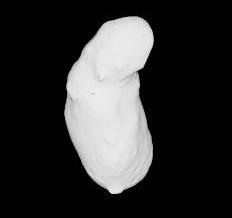
\includegraphics[width = \textwidth, height = 2in]{fig/final_figures_108/unproc_ito.jpg}
    \caption{Unprocessed Itokawa Image}
\end{subfigure}
\hfill
\begin{subfigure}{0.4\textwidth}
    \centering
    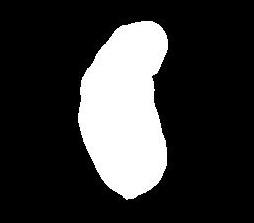
\includegraphics[width = \textwidth, height = 2in]{fig/final_figures_108/flat_thresh_ito.jpg}
    \caption{Processed Itokawa Image}
\end{subfigure}
\end{figure}
\\With a preprocessed, thresholded image, the next step is to apply an edge detection function in order to differentiate the silhouette from the background of space. The function used here is the Canny operator, which can be tuned for sensitivities that correspond to the level of detail desired{Canny1986}. The Canny algorithm applied via Matlab function involves several steps as follows. The first step is to apply another Gaussian filter to smooth the image and thus reduce noise for calculating the edge locations. The equation for the Gaussian kernel applied to the image is below, for an image of size (2k+1)x(2k+1):

\begin{equation}
    H_{ij} = \frac{1}{2\pi \sigma^2} exp\Big(-\frac{(i-(k+1))^2 + (j-(k+1)^2}{2\sigma^2}\Big); 1 \leq i, j \leq (2k+1)
\end{equation}

After the Gaussian noise reduction kernel has been applied, the function needs to find the intensity gradients in the image in order to identify locations of possible edges. The Canny algorithm uses four filters to find four different directions of gradients: vertical, horizontal, and two different diagonal directions. The edge gradient and associated direction is given by the equation which considers both the gradient in the x dimension and the y dimension. 
\begin{equation}
    G = \sqrt{G_x^2 + G_y^2}
\end{equation}
\begin{equation}
    \Theta = tan^{-1}\frac{G_y}{G_x}
\end{equation}
After the gradient is calculated over the image, the desired thresholding factor is applied to eliminate edges of very low or high intensity. In this approach, it is typical to eliminate a large proportion of low intensity edges which, in the particular data sets applied, corresponds to ridges and boulder shadows. At the end of the thresholding process, the algorithm can be confident to a significant degree that is has identified the edge of the objects captured in the given image.

%\begin{figure}[h]
%     \centering
%     \begin{subfigure}[b]{0.32\textwidth}
%         \centering
%         \includegraphics[width=\textwidth,height = \textwidth]{figures/canny_1_1_copy.png}
%         \caption{$T= 0.1, \sigma = 1$}
%         \label{fig:y equals x}
%     \end{subfigure}
%     \hfill
%     \begin{subfigure}[b]{0.32\textwidth}
%         \centering
%         \includegraphics[width=\textwidth,height = \textwidth]{figures/canny_5_1_copy.png}
%         \caption{$T = 0.5, \sigma = 1$}
%         \label{fig:three sin x}
%     \end{subfigure}
%     \hfill
%     \begin{subfigure}[b]{0.32\textwidth}
%         \centering
%         \includegraphics[width=\textwidth,height = \textwidth]{figures/canny_7_1.png}
%        \caption{$T = 0.7, \sigma = 1$}
%         \label{fig:five over x}
%     \end{subfigure}
    
%     \begin{subfigure}[b]{0.32\textwidth}
%         \centering
%         \includegraphics[width=\textwidth,height = \textwidth]{figures/canny_5_1_copy.png}
%         \caption{$T= 0.5, \sigma = 1$}
%         \label{fig:y equals x}
%     \end{subfigure}
%     \hfill
%     \begin{subfigure}[b]{0.32\textwidth}
%         \centering
%         \includegraphics[width=\textwidth,height = \textwidth]{figures/canny_5_5.png}
%         \caption{$T = 0.5, \sigma = 5$}
%         \label{fig:three sin x}
%     \end{subfigure}
%     \hfill
%     \begin{subfigure}[b]{0.32\textwidth}
%         \centering
%         \includegraphics[width=\textwidth,height = \textwidth]{figures/canny_5_10.png}
%         \caption{$T = 0.5, \sigma = 10$}
%         \label{fig:five over x}
%     \end{subfigure}
%        \caption{Different Threshold Levels for Canny Edge Detection on Itokawa Image}
%        \label{fig:three canny}
%\end{figure}
\begin{figure}[h!]
    \centering
    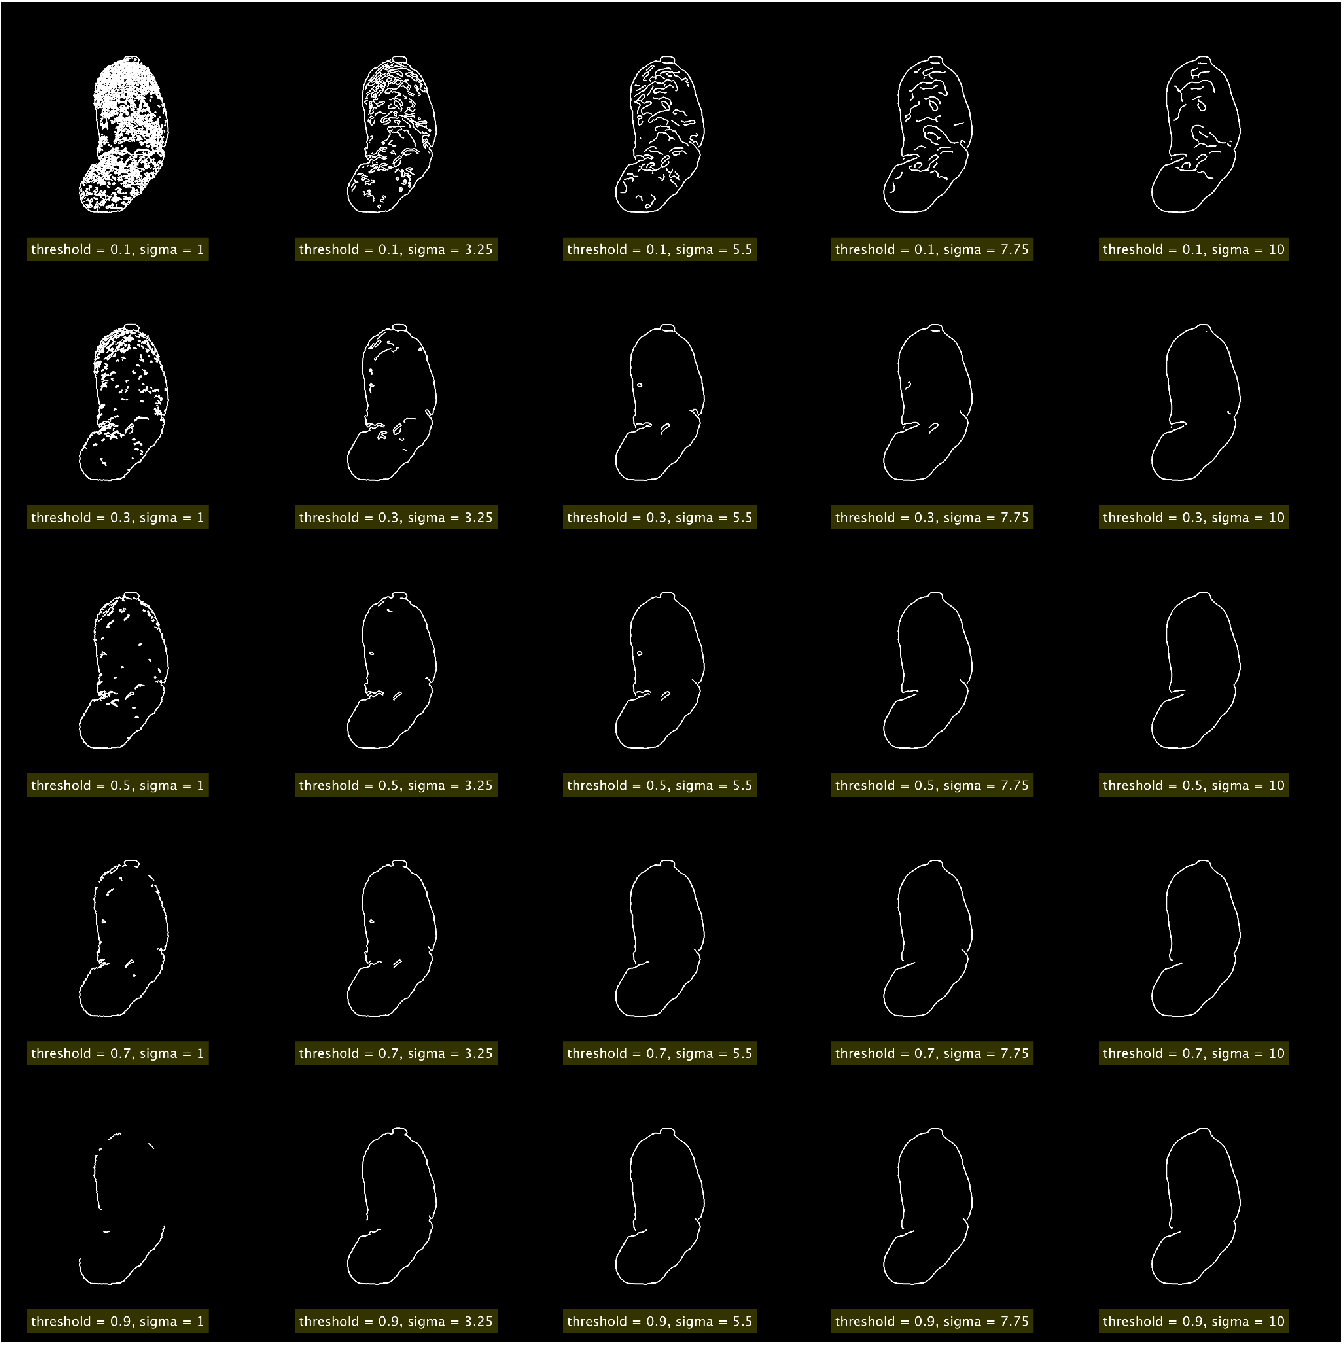
\includegraphics[width = \textwidth]{fig/tiled_canny_test.png}
    \caption{25 Examples of Canny Parameters and Impact on Edge Detection}
    \label{fig:tiled_canny}
\end{figure}
\begin{wrapfigure}[15]{l}{0.4\textwidth}
    \centering
    \vspace{-10pt}
    \captionsetup{justification=centering}
    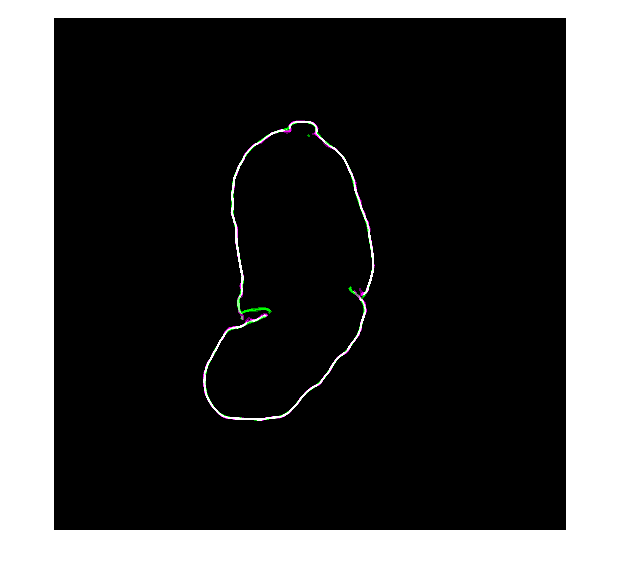
\includegraphics[width = 0.4\textwidth]{fig/overlay_canny_correctparameters.png}
    \caption{Four Edge Results Overlaid in Image Space}
    \label{fig:overlay}
\end{wrapfigure}
In order to capture the edge, the Canny operator was tested for effectiveness over many threshold and standard deviations. Examples of these results are given in Fig. \ref{fig:tiled_canny}, which present the extremes that the function is capable of capturing from the typical asteroid image. The selected values for edge processing were T=0.5 and $\sigma$ = 5. Combined with the previous thresholding steps that output a flat mask, this operator has no issue identifying an appropriate edge for silhouette finding. After the edge is identified, the points are sorted in unit circle order, beginning at the traditional +x axis and moving counter-clockwise in the (u,v) plane. Each image is subsampled to contain an evenly spaced set of points from the full edge result. This is one way in which the data density is reduced for the purpose of faster processing. The original Canny edge output represents each pixel identified as an edge, which can be thousands of data points. 





Taking the four best results from the Canny investigation above, they are overlaid in Fig. \ref{fig:overlay}, to show that differing parameters still provide similar results. The difference between each output is only measured by a few pixels, therefore it can be assumed that the ultimate shape results will not be majorly affected by changing the Canny parameters, as long as the parameters implemented have met the original requirement of identifying only the silhouette and excluding internal features. 

After identifying the silhouette in the image frame and thus in the 3-D camera frame with the addition of the range dimension, the points must be translated into the 3-D body frame which is predefined and known prior to processing. This is an assumption made based on the expected capability to obtain lightcurve information both on the ground and early in the flight plan which will inform about the spin pole and allow for a definition of the body frame to be made. However, for the purposes of this work, the body frame is accessed via SPICE and from scientific convention {Fujiwara2006}{Scheeres2006}.This transformation allows each image to be considered in the body frame against one another, which is what enables the ray trimming process. The points are extended towards and away from the camera direction with the center of the ray corresponding to the originally identified edge point. %include figure of points-> 3d points in body frame -> rays in body frame (use two images for 3d ability)
\subsection{Terminator and Limb Discrimination}
\begin{wrapfigure}[15]{r}{0.4\textwidth}
    \centering
    \vspace{-25pt}
    \captionsetup{justification=centering}
    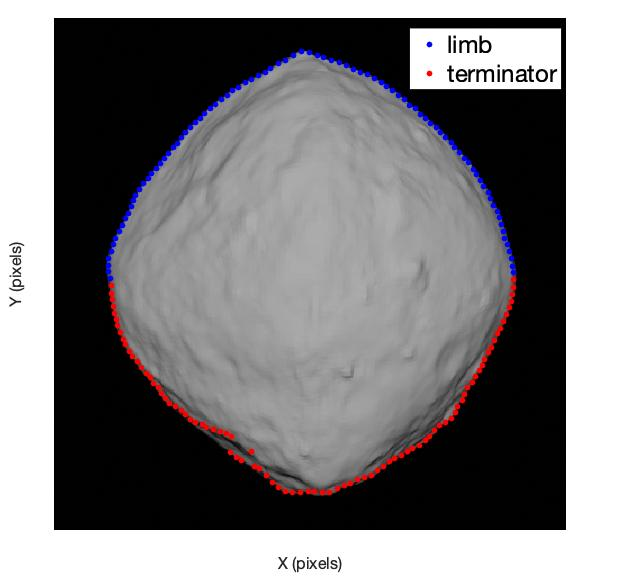
\includegraphics[width = 0.39\textwidth]{fig/limb_term_bennu_correct.jpg}
    \caption{Limb and Terminator in Bennu Mission Image}
    \label{fig:limbwterm}
\end{wrapfigure}
One major known quantity in any space mission is the direction of the sun vector. This is increasingly important for a small body in which the whole shape can be observed along with the terminator, which is dependent on the relationship between the body, the camera, and the sun positions. In this work, it is assumed that there is perfect knowledge of the sun location and thus the unit vector corresponding to the sun direction in the body and image frames. This state allows for a calculation of the phase angle which becomes crucial when differentiating a limb versus a terminator in an image of a body that is only partially lit. The knowledge of the sun unit vector in the camera frame allows for simple vector products to separate the edge points which are facing the sun and the points which are on the opposing side. %add more description here


\subsection{Ray Generation and Trimming}


The silhouettes have been identified and placed in their assumed positions in the bodycentric frame of the target, and now the next step is to extend these points into rays which will concentrically constrain the surface {Mcmahon2018}. The reason why the rays are necessary is that the points themselves may be misaligned, contain outliers, or possibly not hold enough information to solve for a reasonable resolution of the surface. Extending our points into rays which will be trimmed based on intersections and subsampled allows for more detail without requiring more information. 

%\begin{figure}[h!]
%    \centering
%    \begin{subfigure}[b]{0.32\textwidth}
%        \centering
%        \vcenter{\includegraphics[width = 0.8\textwidth,height = %1.2in]{figures/edge_points_1image.png}}
%        \caption{Original Edge Points in Camera Frame}
%    \end{subfigure}
%    \hfill
%    \begin{subfigure}[b]{0.32\textwidth}
%        \centering
%        \vcenter{\includegraphics[width = \textwidth, height = %1.5in]{figures/one_rays.png}}
%        \caption{Rays: One Image}
%    \end{subfigure}
%    \hfill
%    \begin{subfigure}[b]{0.32\textwidth}
%        \centering
%        \vcenter{\includegraphics[width = \textwidth, height = %1.5in]{figures/two_rays.png}}
%        \caption{Rays: Two Images}
%    \end{subfigure}
%    \caption{Ray Population Process}
%    \label{fig:intensity}
%\end{figure}
\\
The rays are described using a line equation to characterize them in 3D body frame space. The equation of the line segments is as follows for i number of rays $l$ in each view. 
\begin{equation}
    l_i = l_{i,0} + \eta L \hat{r}
\end{equation}


In the above equation, $l_{i,0}$ is the initial point of the ray, $\eta$ is the scale factor from 0 to 1 describing how far along the rays length it's been trimmed (between 0 and 100 percent), L is the length of the pretrimmed ray, and $\hat{r}$ is a generic unit view direction. For this investigation, the original ray length L is set to 2km, centered at the identified edge point and extended towards and away from the camera for limb points, with terminator points at a slight rotation proportional to the phase angle. The $\eta$ factor is calculated after finding all intersections between each limb plane and trimming each ray down to it's likely surface section, and this procedure will be described in later sections.
\begin{wrapfigure}[14]{l}{0.5\textwidth}
    \centering
    \vspace{-10pt}
    \captionsetup{justification=centering}
    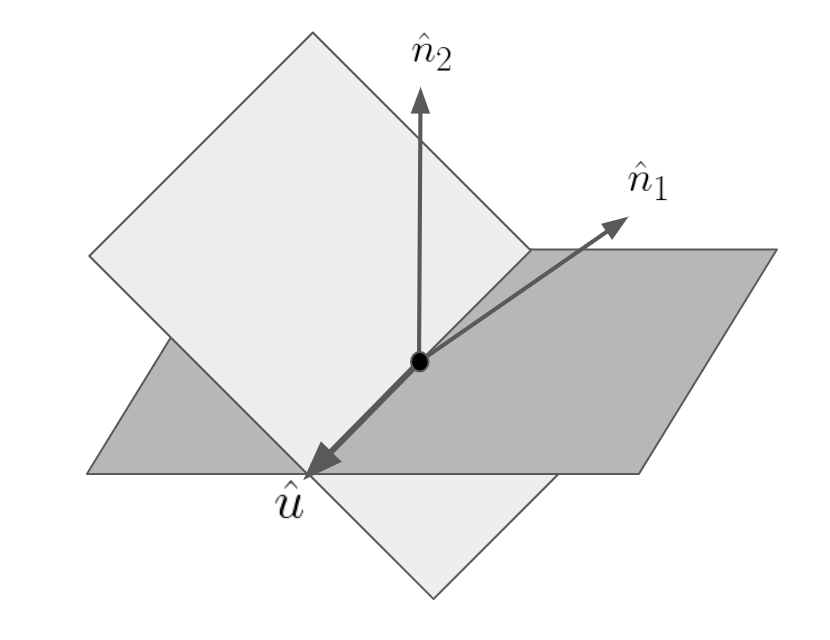
\includegraphics[width = 0.5\textwidth]{fig/planes_intersect.png}
    \caption{Geometry of Two Intersecting Planes}
    \label{fig:two_intersect}
\end{wrapfigure}
\\With a sample of $N_p$ edge points, there can be $N_p$ number of planar quadrilaterals formed by connecting each adjacent edge point as seen in Fig. \ref{fig:twoplanes}, and calculating its surface normal direction with the following equation:
\begin{equation}
\hat{n}_k = \frac{\hat{r} \times (l_{i+1,0} - l_{i,0})}{|\hat{r} \times (l_{i+1,0} - l_{i,0})|}
\end{equation}



The planar quadrilaterals will be referred to as patches in the following discussion. These patches have an associated normal vector, and two rays which describe the lines in the $\hat{r}$ direction. Processing this information in a batch method, all of the rays are iterated through to find where each plane intersects with another plane from the found silhouettes. The locations of the intersection, along with the percentage along the ray that the location is identified, are saved and then evaluated to find where the rays need to be trimmed away. The line of intersection between two planes in 3D space exists if the cross product of the two normal vectors associated with each plane is nonzero. If $n_1 \times n_2 = 0$, then the two planes in question are parallel and will be ignored. In the implementation presented here, the threshold for a nonzero parallel evaluation is that the magnitude of the cross product of the normal vectors is above $1\times 10^{-10}$. The line of intersection itself also lies along the cross product of the two normal vectors. If an intersection can be found, the $\eta$ value corresponding how much of the line should be kept is saved, and the rest of the line is trimmed and the equation of this specific line is updated to go between $\eta$ length and the other remaining end for the next iteration. Now the direction vector of the intersection line can be founds using the normal vectors of the two planes, as shown in Eq.3. The variable $m$ gives the direction of slope, and a point on the line is found numerically, which corresponds to b, and from there a whole line equation is given in $y = mx + b$ form. 
\begin{equation}
    m = \frac{\hat{n}_1 \times \hat{n}_2}{|\hat{n}_1 \times \hat{n}_2|}
\end{equation}

%now describe the trimming procedure

The results from the line intersection calculations are many line equations describing the unit vector corresponding to the direction of the intersection line, the end points of the original rays, and the points corresponding to the physical end of the intersection line for these finite patches. The next step is to evaluate which parts of the ray must be trimmed away based on the identification of a crossing, and which portions of the ray are kept. 
%above I need to include some math corresponding to the trimming procedure - the trim happens where the normal vectors switch signs along the intersection rays ????
\begin{figure}
    \centering
    \begin{subfigure}[b]{0.49\textwidth}
        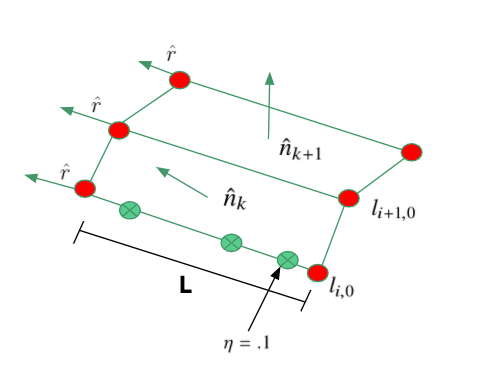
\includegraphics[width = \textwidth]{fig/twoplanes.png}
        \caption{Two adjacent edge planes with sampled points along the line of length L}
    \end{subfigure}
    \hfill
    \begin{subfigure}[b]{0.49\textwidth}
        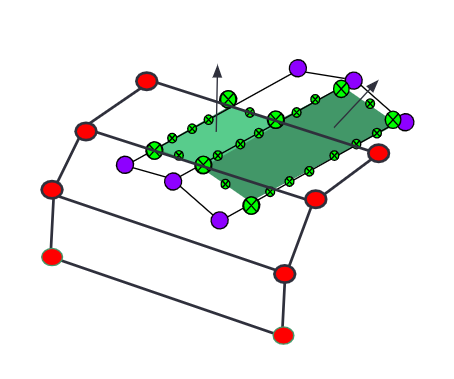
\includegraphics[width = \textwidth]{fig/intersecting_planes.png}
        \caption{Planes and their associated normal vectors: Two observations}
    \end{subfigure}
    \caption{Geometric Depiction of Patch Crossing Calculations}
    \label{fig:twoplanes}
\end{figure}
The algorithm sorts the points along the intersection ray based on the percent along the ray which they fall, and then locates where the calculated projected normal directions switch in sign. This switch is the indicator of an intersection with another limb patch, and therefore serves to show where the ray must be trimmed.
In Fig.\ref{fig:line_pts}, the point identified is $20\%$ along the intersection ray, with a positive normal direction. The point which will delineate the trimmed portion of the ray is at $50\%$ along the original ray, where the surface normal vectors have switched. The derivation of a surface normal direction is crucial for the process of delineating which points intersect on the body and which points intersect off the body and therefore should be discarded. The points that theoretically constrain the surface are what's left after a ray has been processed to find intersections meant to eliminate the points that extend too far. 
\\ As the views are iterated over, the plane intersections are examined and a check is performed to find out if the plane segments are on the inside or outside of the silhouette using the calculation of the surface normal from Eq.3. The segments that are kept are not intersected at all, and therefore must represent our knowledge of where the surface is depending on the resolution of our observation data. As shown in Fig.\ref{fig:twoplanes}, one view overlaps with another view and two patches are found. One patch is formed from coplanar limbs and the green points represent the intersections saved. The other patch only intersects the first view on one side, so only one side of the original limb gets trimmed down and resampled. Both of the resulting patches, shown by the green planes, have new normal directions based on the normal directions of the limbs that were intersecting to form them. 
\begin{wrapfigure}[7]{r}{0.5\textwidth}
    \centering
    \vspace{-10pt}
    \captionsetup{justification=centering}
    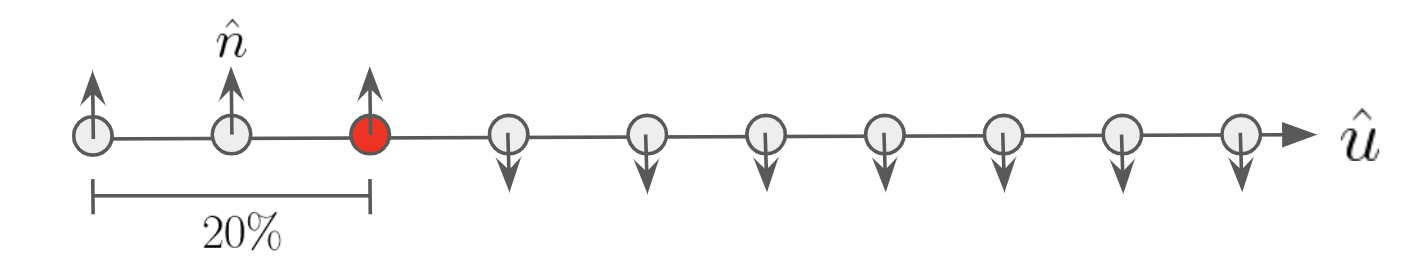
\includegraphics[width = 0.5\textwidth]{fig/line_pts_norms.png}
    \caption{Intersection Ray from Two Patches - Ten Sampled Points and Associated Ray Normals}
    \label{fig:line_pts}
\end{wrapfigure}
\indent After iterating through each view and trimming off the pieces of the rays that become intersected by another silhouette, the algorithm saves the remaining points as a point cloud output result. The segments of the original ray that are kept are the ones that were never intersected. This evaluation is strict and a misidentified edge point could result in the trimming of necessary and correct surface data. This drawback is kept in mind during the tuning procedure of the Canny edge detection function, which is designed to be the least sensitive and therefore refined to only identify true edge points. Depending on the range of the observations about the target body, the surface can be resolved to different magnitudes. It is possible to localize using single-view geometry because of the assumption that range is known. Without this assumption, a multiple-view refinement of location using the coordination of edge points along epipoles within the image frame would be required. This estimation capability can easily be implemented in future iterations of this work in order to reduce assumptions and provide further autonomy to the method. However, in the scope of this work, it is assumed that the attitude and range are known quantities for our spacecraft. If a full equatorial survey is able to be conducted, the resulting model will have more data and thus can be further refined by our method compared to a survey with less frequent observations taken. In the test cases presented in this paper, simulated data was used to represent an optimal scenario of observational ability. Using Blender {blender}, the case of a $0^\circ$ phase angle could be simulated for maximum limb brightness and the elimination of a terminator. Data sets were collected for both Itokawa and Bennu, to examine the individual challenges of mapping an irregular shaped body versus a symmetric body. 




\subsection{Surface Reconstruction}
The final result of ray trimming will be the 3D locations of points on the surface of the shape as observed by our simulated imaging procedure. Each point will have an associated normal vector. The next step is to form a closed surface for comparison to the published shape models of the bodies in question. This surface calculation is performed via the boundary function in Matlab, which is a function that returns a single conforming boundary around the points provided. This function utilizes a version of the alphaShape calculation procedure, but it differs by shrinking towards the interior of the hull in order to capture concavities in the surface. The returned result of this function is a K-size set of triangular facet point indices. 

%show figures of the solved shape 




\subsection{Usage of Infrared Images}
% Reasons for using IR
One major issue arising from the optical Silhouette approach is that the center of the body can be misidentified for phase angles not close to zero. This results in the less accurate modeling even in cases where the terminator is used. Moreover, at non-zero phase angles, only partial silhouette is observed which at best results in a trade-off with the silhouette obtained from the terminator. 

% NOTE: last sentence may need to be justified or just removed

To address the drawbacks with the optical approach, one can turn to the infrared spectrum. Due to the temperature difference between the celestial body and the background of space, the entire silhouette can be extracted regardless of the phase angle. Having the entire silhouette also alleviates the center finding bias that was observed in the optical only method. The infrared silhouette can augment the information found in the optical limb and terminator to produce a more accurate shape model of the body.
% Method for obtaining IR images
\subsection{Simulated Infrared Image Procedure}
Under the assumption that the infrared images are robust to any phase angle, we can assume that the entire silhouette of the body will be visible at all times. A simple way to model such a silhouette is to set the light direction along the same line of sight as the spacecraft and generate the images in the optical spectrum. This is accomplished using the Blender software using similar setup as in the optical approach. 
% Show images
\begin{figure}[h!]
     \centering
     \begin{subfigure}[b]{0.49\textwidth}
         \centering
         \includegraphics[width=0.7\textwidth,height = 0.7\textwidth]{figures/bennu_IR_rawImage.png}
         \caption{Simulated Bennu Infrared Image in Blender}
         \label{fig:bennuRawIRImage}
     \end{subfigure}
    \hfill
     \begin{subfigure}[b]{0.49\textwidth}
         \centering
         \includegraphics[width=0.7\textwidth,height = 0.7\textwidth]{figures/itokawa_IR_rawImage.png}
         \caption{Simulated Itokawa Infrared Image in Blender}
         \label{fig:three sin x}
     \end{subfigure}
        \caption{}
        \label{fig:itokawaRawIRImage}
\end{figure}
% IR silhouette
From these images, a silhouette can be by first thresholding the image such that the background appears to be black and the body appears to be white. The silhouette is then computed by noting the first and last non-black pixel in each row and column.
% add center finding section
The bias noted earlier from the center finding algorithm can be mitigated.
% figure comparing the bias reduction between optical and infrared silhouettes
% link to optical 
These silhouettes are used in conjunction with the optical limb and terminator lines to estimate the shape of the body.
% Show Thresholded images
\begin{figure}[h!]
     \centering
     \begin{subfigure}[b]{0.49\textwidth}
         \centering
         \includegraphics[width=0.7\textwidth,height = 0.7\textwidth]{figures/bennu_IR_threshImage.png}
         \caption{Thresholded Bennu Infrared Image in Blender}
         \label{fig:bennuThreshIRImage}
     \end{subfigure}
    \hfill
     \begin{subfigure}[b]{0.49\textwidth}
         \centering
         \includegraphics[width=0.7\textwidth,height = 0.7\textwidth]{figures/itokawa_IR_threshImage.png}
         \caption{Thresholded Itokawa Infrared Image in Blender}
         \label{fig:itokawaThreshIRImage}
     \end{subfigure}
        \caption{}
        \label{fig:rawIRImage}
\end{figure}
% show silhouette
\begin{figure}[h!]
     \centering
     \begin{subfigure}[b]{0.49\textwidth}
         \centering
         \includegraphics[width=0.7\textwidth,height = 0.7\textwidth]{figures/bennu_IR_silhouette.png}
         \caption{Bennu Infrared Silhouette in Blender}
         \label{fig:bennuSilIRImage}
     \end{subfigure}
    \hfill
     \begin{subfigure}[b]{0.49\textwidth}
         \centering
         \includegraphics[width=0.7\textwidth,height = 0.7\textwidth]{figures/itokawa_IR_silhouette.png}
         \caption{Itokawa Infrared Silhouette in Blender}
         \label{fig:itokawaSilIRImage}
     \end{subfigure}
        \caption{}
        \label{fig:rawIRImage}
\end{figure}
\section{Results}

The results shown here represent the implementation of the above procedure on several data sets of multiple bodies. The data sets encompass simulated and actual mission imagery. The goal of the shape modeling method is to make a three-dimensional hull from the measurements of the silhouette in multiple images. Below are the models resultant of this procedure, and following sections will compare them to the truth model in which the data was derived from or the most appropriate shape model for the body in question. These shape models are representative of a batch implementation of onboard shape modeling with idealized conditions and assumptions of perfect state and frame knowledge.
\begin{wrapfigure}[16]{r}{0.5\textwidth}
    \centering
    \vspace{-10pt}
    \captionsetup{justification=centering}
    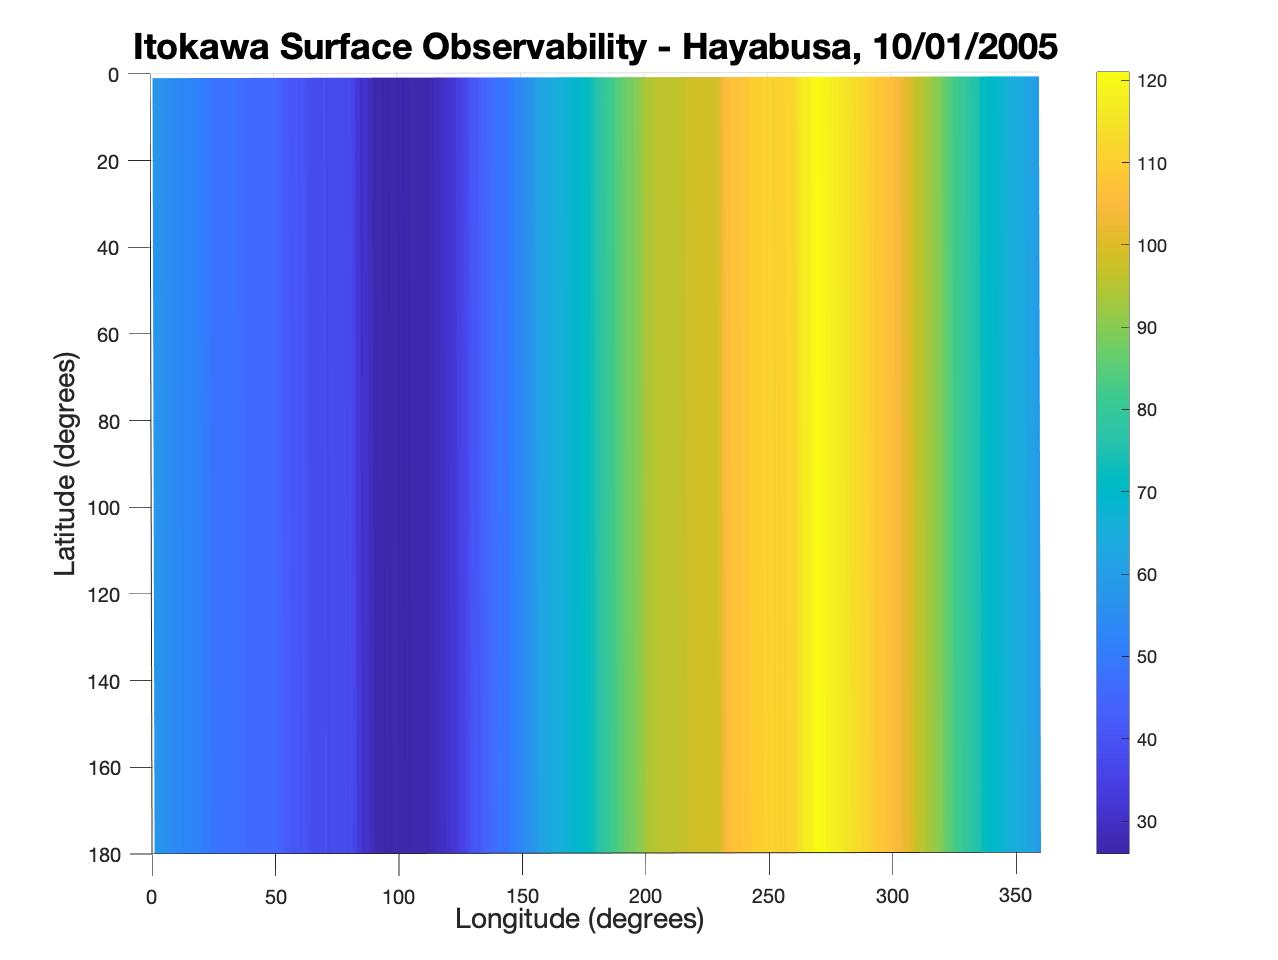
\includegraphics[width=0.5\textwidth,height = 2in]{fig/hayabusa_obs_heatmap.jpg}
    \caption{Range of Image Observations in Optimal Hayabusa Data Set (133 Images). Color corresponds to Number of Surface Observations}
    \label{fig:surf_obs_hayabusa}
\end{wrapfigure}


In the limb-only test case, the same images from the $10^{\circ}$ asteroid examples were processed, however, the terminator information was left out. This is to provide a comparison to the original test case, which utilized the terminator information to get a better mapping of the body. Comparing the statistics of the two approaches, it can be derived whether the inclusion of terminator information improves or worsens the resultant model. If it is able to improve upon the estimate made with just the limb information, then this method has accurately modeled the terminator and can use more points per image than limb-only cases. Successfully using the terminator information also reduces the number of images required before a full-coverage shape model can be developed. However, if the model developed with only limb information is a better surface comparison to the truth model, then it is known that there is a drawback to including the terminator information which is based in a biased approach to differentiating the limb and terminator and centering the silhouette points in the image.

The goal of additional test cases using more frequent images was to see the relationship between image density over the surface and model accuracy. Observing a denser amount of the target surface provides more data on the limb which could provide more precision for surface features such as boulders and craters. As compared to the previous simulated test cases where images were captured at every $5^{\circ}$ of rotation about the body spin pole, this test case examines the results from a set of 120 images taken at every $3^{\circ}$ about the body spin pole from the perspective of a stationary camera in the body rotational frame. 



\subsection{Simulated Convex Modeling}
This is where the Bennu results will go.



\subsection{Simulated Non-Convex Modeling}
This is where Itokawa results will go.

\subsection{OSIRIS-REx Mission Modeling}

\subsection{Hayabusa Mission Modeling}
\subsection{Infrared and Visual Data Fusion}
The procedure for combining the visual and IR representations of our data is similar to processing two different image sets of the same body simultaneously. The visual data is presented with a phase angle greater than zero, therefore a terminator is visible. In the infrared spectrum, there is no terminator as we assume the full body limb is visible to the IR spectrometer. 

\section{Analysis}
\subsection{Error Evaluation}
The models generated with the limb-trimming method have been compared to mission-derived truth models of the same bodies. The 101955 Bennu shape model used for comparison is sourced from data during the approach phase of the OSIRIS-REx mission, and was made available publicly in November 2018{}. This model has a resolution of 6m over the surface. The 25143 Itokawa shape model used for comparison is the Gaskell shape model produced with Hayabusa with a resolution of 49,152 facets{Gaskell2004}. A surface comparison between two shape models is performed using a Distance from Reference Mesh function, which calculates the closest distance from the reference mesh, or truth model, to the measured mesh, which is the model produced via limb trimming. The distance is left signed to appropriately characterize under- or over-estimated volumes. 


\begin{table*}[h!]
\centering
     \begin{tabular}{|c||c|c|c|c||c|c|}
     \hline
     \multicolumn{1}{|c||}{}&
     \multicolumn{4}{c||}{Point Cloud Dimensions}&
     \multicolumn{2}{c|}{Surface Reconstruction}\\
     \hline
           \textbf{Test Case}& \textbf{$\#$ of Points} & \textbf{x (m)} & \textbf{y (m)} & \textbf{z (m)} & \textbf{Mean Error (m)} & \textbf{RMS (m)} \\
          \hline
          
          Bennu Truth Model{Barnouin2019} & 25350 & 563.3& 541.4& 495.5 & N/A  & N/A\\
          \hline
          
          \hline
          
          Itokawa Truth Model{gaskell_ito} & 24578 & 560.5& 305.3& 243.5 & N/A  & N/A\\
          \hline
     \end{tabular}
     \caption{Comparison of Shape from Silhouette Model Results to Truth Models}
\end{table*}

\section{Discussion}

\section{Conclusion and Further Work}


\section{Acknowledgments}

This material is based upon work supported by the National Science Foundation Graduate Research Fellowship under Grant No. DGE 1650115. Any opinion, findings, and conclusions or recommendations expressed in this material are those of the authors and do not necessarily reflect the views of the National Science Foundation.




\end{document}
